\documentclass{article}
\usepackage{enumitem}
\usepackage{graphicx}
\usepackage{amsmath}
\usepackage{amssymb}
\usepackage{microtype}
\usepackage{vwcol}  
\usepackage{multicol}
\usepackage{cancel}
\usepackage[top=1cm, left=1.5cm, bottom=0.5cm, right=1.5cm]{geometry}
\usepackage{mathrsfs}
\usepackage{xcolor}
\usepackage{enumitem}
\usepackage{comment}
\usepackage{hyperref}
\usepackage{paracol}
\usepackage{pdfpages}



% Comandos personalizados
\newcommand{\combinat}[2]{\begin{pmatrix} {#1} \\ {#2} \end{pmatrix}}
\newcommand{\magn}[1]{\left[#1 \right]}
\newcommand{\lpn}[1]{\mathscr{L}^{-1}\left\{#1\right\}}
\newcommand{\lp}[1]{\mathscr{L}\left\{#1\right\}}

\newcommand{\frt}[1]{\mathscr{F}\left\{#1\right\}}
\newcommand{\frtn}[1]{\mathscr{F}^{-1}\left\{#1\right\}}

\newcommand{\evalat}[2]{\left. #1 \right|_{{#2}}}
\newcommand{\arccsc}{\operatorname{arccsc}}
\newcommand{\arcsec}{\operatorname{arcsec}}
\newcommand{\arccot}{\operatorname{arccot}}

%    This allows to reference formulas as Section.Subsection. Formula
\newcounter{fmSubSec}[section]
\newcounter{fmCounter}[fmSubSec]
\newcommand{\theformulaCounter}{\arabic{section}.\arabic{fmSubSec}.\arabic{fmCounter}}

\newlist{itemform}{itemize}{1}
\setlist[itemform]{
  label=\textcolor{magenta}{-},
  ref=(\theformulaCounter),
  leftmargin=*,
  noitemsep,
  topsep=0pt,    before=\let\olditem\item\def\item{\stepcounter{fmCounter}\olditem}
}

% Comando para subsecciones (conservando tu nombre)
\newcommand{\fmSubSec}[1]{%
  \stepcounter{fmSubSec}%
  \setcounter{fmCounter}{0}%
  \subsection{#1}%
}

\newenvironment{Figure}
  {\par\medskip\noindent\minipage{\linewidth}}
  {\endminipage\par}
\usepackage{background}

\backgroundsetup{contents=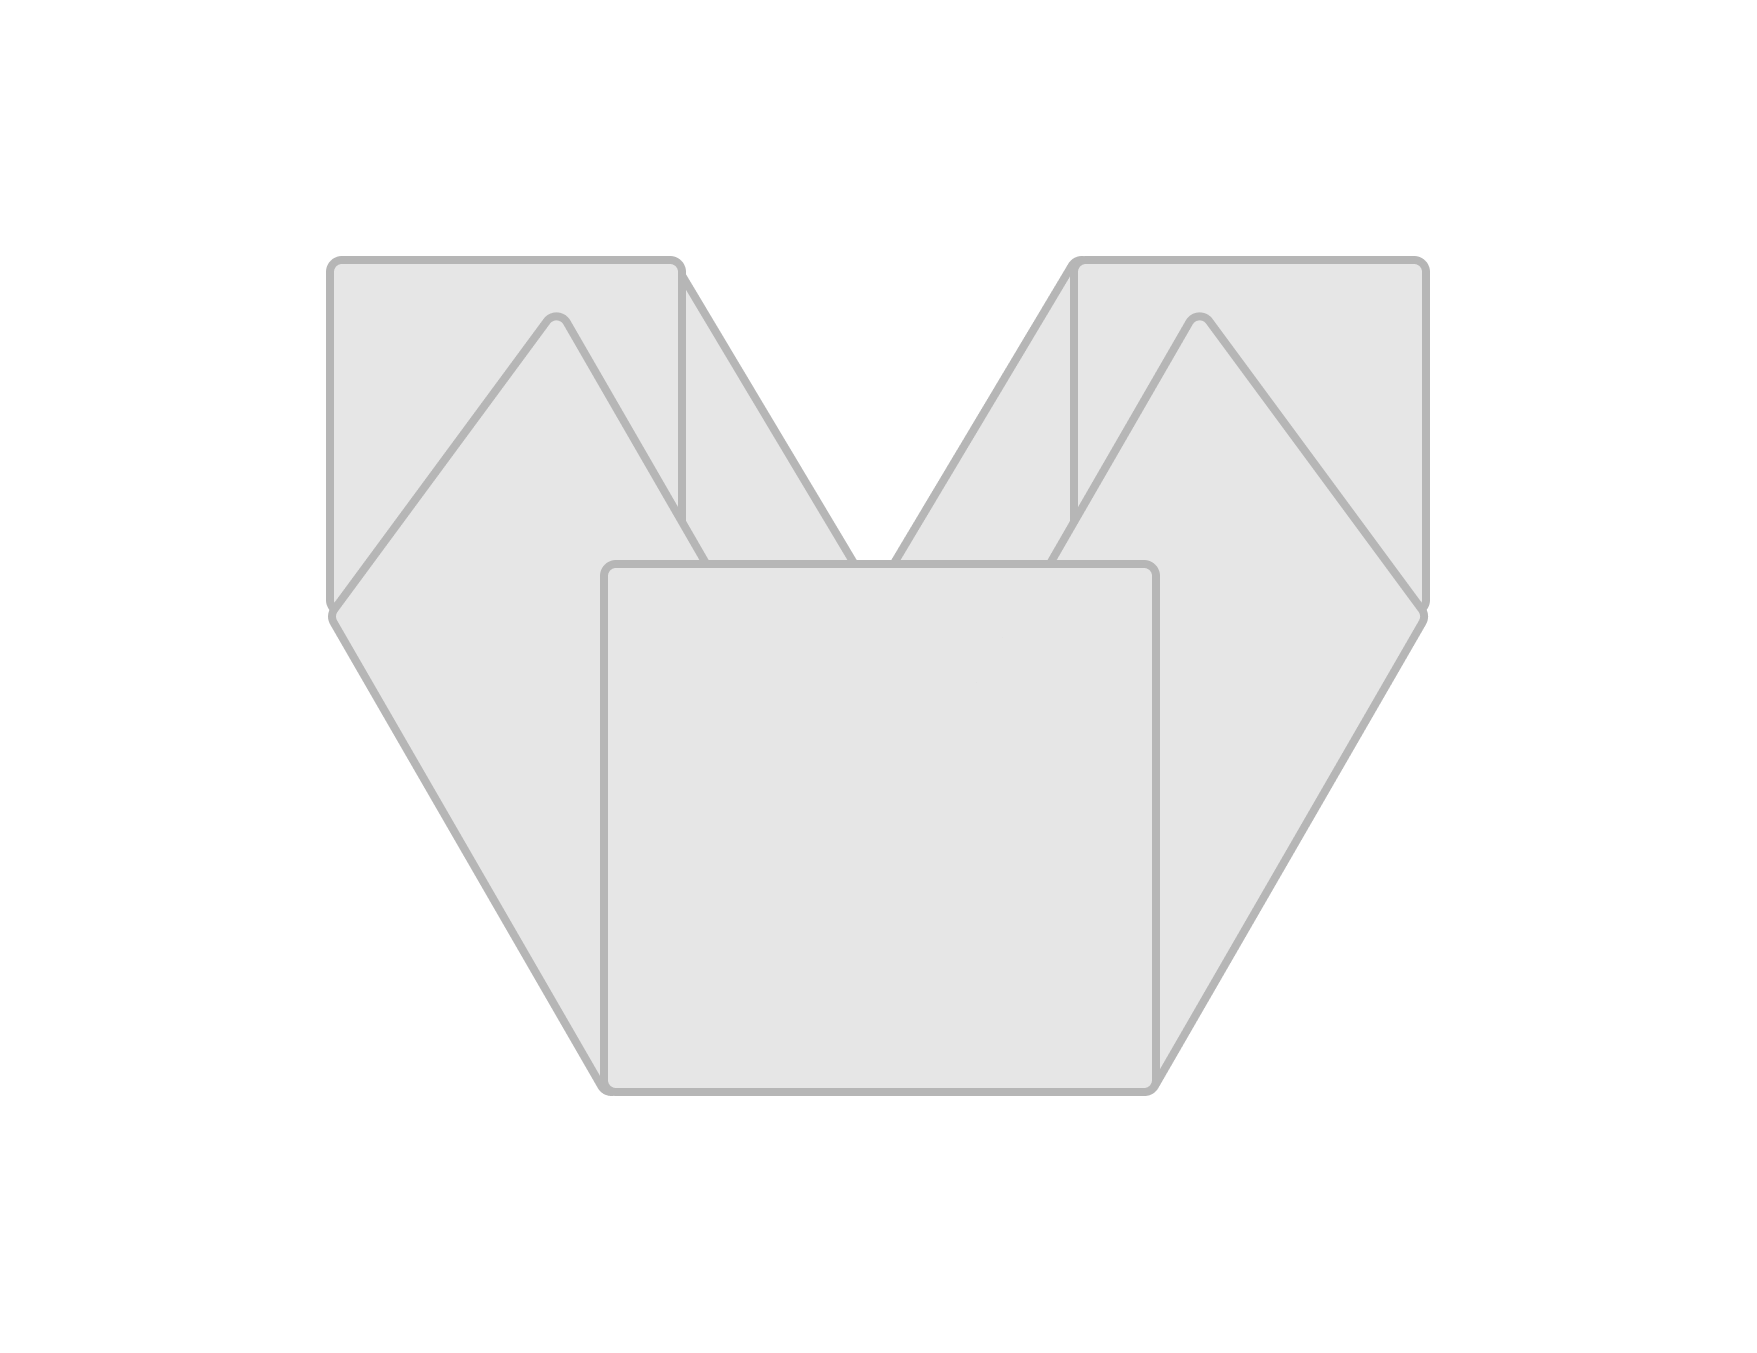
\includegraphics{ALUDAS.png}, scale=1, opacity=0.4,angle =0}

\hypersetup{
    colorlinks=true,
    linkcolor=purple,
    filecolor=magenta,      
    urlcolor=cyan,
    pdftitle={Ultimate Madaf Formulary},
    pdfauthor={Das Reyes},
    bookmarks=true,
    pdfpagemode=FullScreen,
}
\begin{document}         \begin{multicols}{2}
                            \section{Ecuaciones Diferenciales}

                            \fmSubSec{Clasificación por Orden}
                            \begin{itemform}
                            \item \textbf{1er orden}: $\dfrac{dy}{dx} = f(x,y)$
                            \item \textbf{2do orden}: $\dfrac{d^2y}{dx^2} = f\left(x,y,\dfrac{dy}{dx}\right)$
                            \item \textbf{Orden n}: $F\left(x,y,y',\dots,y^{(n)}\right) = 0$
                            \item \textbf{Lineal}: $a_n(x)y^{(n)} + \cdots + a_0(x)y = g(x)$
                            \end{itemform}

                            \fmSubSec{Métodos para EDOs 1er Orden}
                            \begin{itemform}
                            \item \textbf{Separables}:
                              $$\dfrac{dy}{dx} = \dfrac{f(x)}{g(y)} \Rightarrow \int g(y)dy = \int f(x)dx$$

                            \item \textbf{Lineales}:
                              $$y' + P(x)y = Q(x)$$
                              Solución: $y = e^{-\int P dx}\left(\int Q e^{\int P dx}dx + C\right)$

                            \item \textbf{Exactas}:
                              $$Mdx + Ndy = 0 \quad \text{con} \quad \dfrac{\partial M}{\partial y} = \dfrac{\partial N}{\partial x}$$
                              Solución: $\psi(x,y) = C$ donde $d\psi = Mdx + Ndy$

                            \item \textbf{Bernoulli}:
                              $$y' + P(x)y = Q(x)y^n$$
                              Sustitución: $v = y^{1-n}$

                            \item \textbf{Homogéneas}:
                              $$\dfrac{dy}{dx} = F\left(\dfrac{y}{x}\right)$$
                              Sustitución: $v = \dfrac{y}{x}$
                            \end{itemform}

                            \fmSubSec{EDOs Lineales de 2do Orden}
                            \begin{itemize}[leftmargin=*,noitemsep,topsep=0pt]
                              \item \textbf{Homogéneas}:
                                $$ay'' + by' + cy = 0$$
                                Ecuación característica: $ar^2 + br + c = 0$
                                \begin{itemize}[leftmargin=*,noitemsep,topsep=0pt]
                                  \item Raíces reales distintas: $y = C_1e^{r_1x} + C_2e^{r_2x}$
                                  \item Raíz doble: $y = (C_1 + C_2x)e^{rx}$
                                  \item Complejas: $y = e^{\alpha x}(C_1\cos\beta x + C_2\sin\beta x)$
                                \end{itemize}

                              \item \textbf{No homogéneas}:
                                $$ay'' + by' + cy = g(x)$$
                                \begin{itemize}[leftmargin=*,noitemsep,topsep=0pt]
                                  \item \textbf{Coef. Indeterminados}: Para $g(x) = P(x)e^{kx}$
                                  \item \textbf{Variación Parámetros}:
                                    $$y_p = -y_1\int \dfrac{y_2 g}{W}dx + y_2\int \dfrac{y_1 g}{W}dx$$
                                    donde $W = y_1y_2' - y_2y_1'$ (Wronskiano)
                                \end{itemize}
                            \end{itemize}

                            \columnbreak
                            \section{Transformada de Laplace}
                            \fmSubSec{Definición Formal}
                            \begin{itemize}[leftmargin=*,noitemsep,topsep=0pt]

                              \item \textbf{Transformada}:
                                $$\lp{f(t)} = F(s) = \int_0^\infty e^{-st}f(t)dt$$
                                donde $s = \sigma + i\omega$ (variable compleja)

                              \item \textbf{Existencia}: Si $f(t)$ es:
                                \begin{itemize}[leftmargin=*,noitemsep,topsep=0pt]
                                  \item Continua por partes
                                  \item De orden exponencial $\exists M,\alpha$ tal que $|f(t)| \leq Me^{\alpha t}$
                                \end{itemize}
                            \end{itemize}

                            \begin{multicols}{2}

                              \fmSubSec{Transformada}
                              $$
                              \begin{aligned}
                                \lp{1} &= \dfrac{1}{s}\\
                                \lp{t^n} &= \dfrac{n!}{s^{n+1}}\\
                                \lp{e^{at}} &= \dfrac{1}{s - a}\\
                                \lp{\sin(kt)} &= \dfrac{k}{s^2 + k^2}\\
                                \lp{\cos(kt)} &= \dfrac{s}{s^2 + k^2}\\
                                \lp{\sinh(kt)} &= \dfrac{k}{s^2 - k^2}\\
                                \lp{\cosh(kt)} &= \dfrac{s}{s^2 - k^2}\\
                              \end{aligned}
                              $$

                              \columnbreak

                              \fmSubSec{Transformada Inversa}
                              $$
                              \begin{aligned}
                                \lpn{\dfrac{1}{s}} &= 1\\
                                \lpn{\dfrac{n!}{s^{n+1}}} &= t^n\\
                                \lpn{\dfrac{1}{s - a}} &= e^{at}\\
                                \lpn{\dfrac{k}{s^2 + k^2}} &= \sin(kt)\\
                                \lpn{\dfrac{s}{s^2 + k^2}} &= \cos(kt)\\
                                \lpn{\dfrac{k}{s^2 - k^2}} &= \sinh(kt)\\
                                \lpn{\dfrac{s}{s^2 - k^2}} &= \cosh(kt)\\
                              \end{aligned}
                              $$

                            \end{multicols}

                            \fmSubSec{Teoremas Clave}
                            \begin{itemform}
                              \item \textbf{1er Teorema de Traslación}:
                                $$\lp{e^{at}f(t)} = F(s-a)$$

                              \item \textbf{2do Teorema de Traslación}:
                                $$\lp{f(t-a)u(t-a)} = e^{-as}F(s)$$
                                ($u(t-a)$: función escalón)

                              \item \textbf{Derivada n-ésima}:
                                $$\lp{f^{(n)}(t)} = s^n F(s) - \sum_{k=1}^n s^{n-k}f^{(k-1)}(0)$$

                              \item \textbf{Multiplicación por $t^n$}:
                                $$\lp{t^n f(t)} = (-1)^n \dfrac{d^n F(s)}{ds^n}$$

                              \item \textbf{Integración}:
                                $$\lp{\int_0^t f(\tau)d\tau} = \dfrac{F(s)}{s}$$
                            \end{itemform}

                            \subsection*{Aplicación a EDOs}
                            \begin{itemize}[leftmargin=*,noitemsep,topsep=0pt]
                              \item \textbf{Pasos para resolver} $ay'' + by' + cy = g(t)$:
                                \begin{enumerate}[leftmargin=*,noitemsep,topsep=0pt]
                                  \item Aplicar $\lp{}$ a ambos lados
                                  \item Sustituir condiciones iniciales
                                  \item Despejar $Y(s)$
                                  \item Antitransformar usando fracciones parciales
                                \end{enumerate}

                              \item \textbf{Ejemplo clásico}:
                                $$\lp{y'' + \omega^2 y = 0} \Rightarrow Y(s) = \dfrac{sy(0) + y'(0)}{s^2 + \omega^2}$$
                            \end{itemize}
                    
                                              \end{multicols}
                    \newpage
                    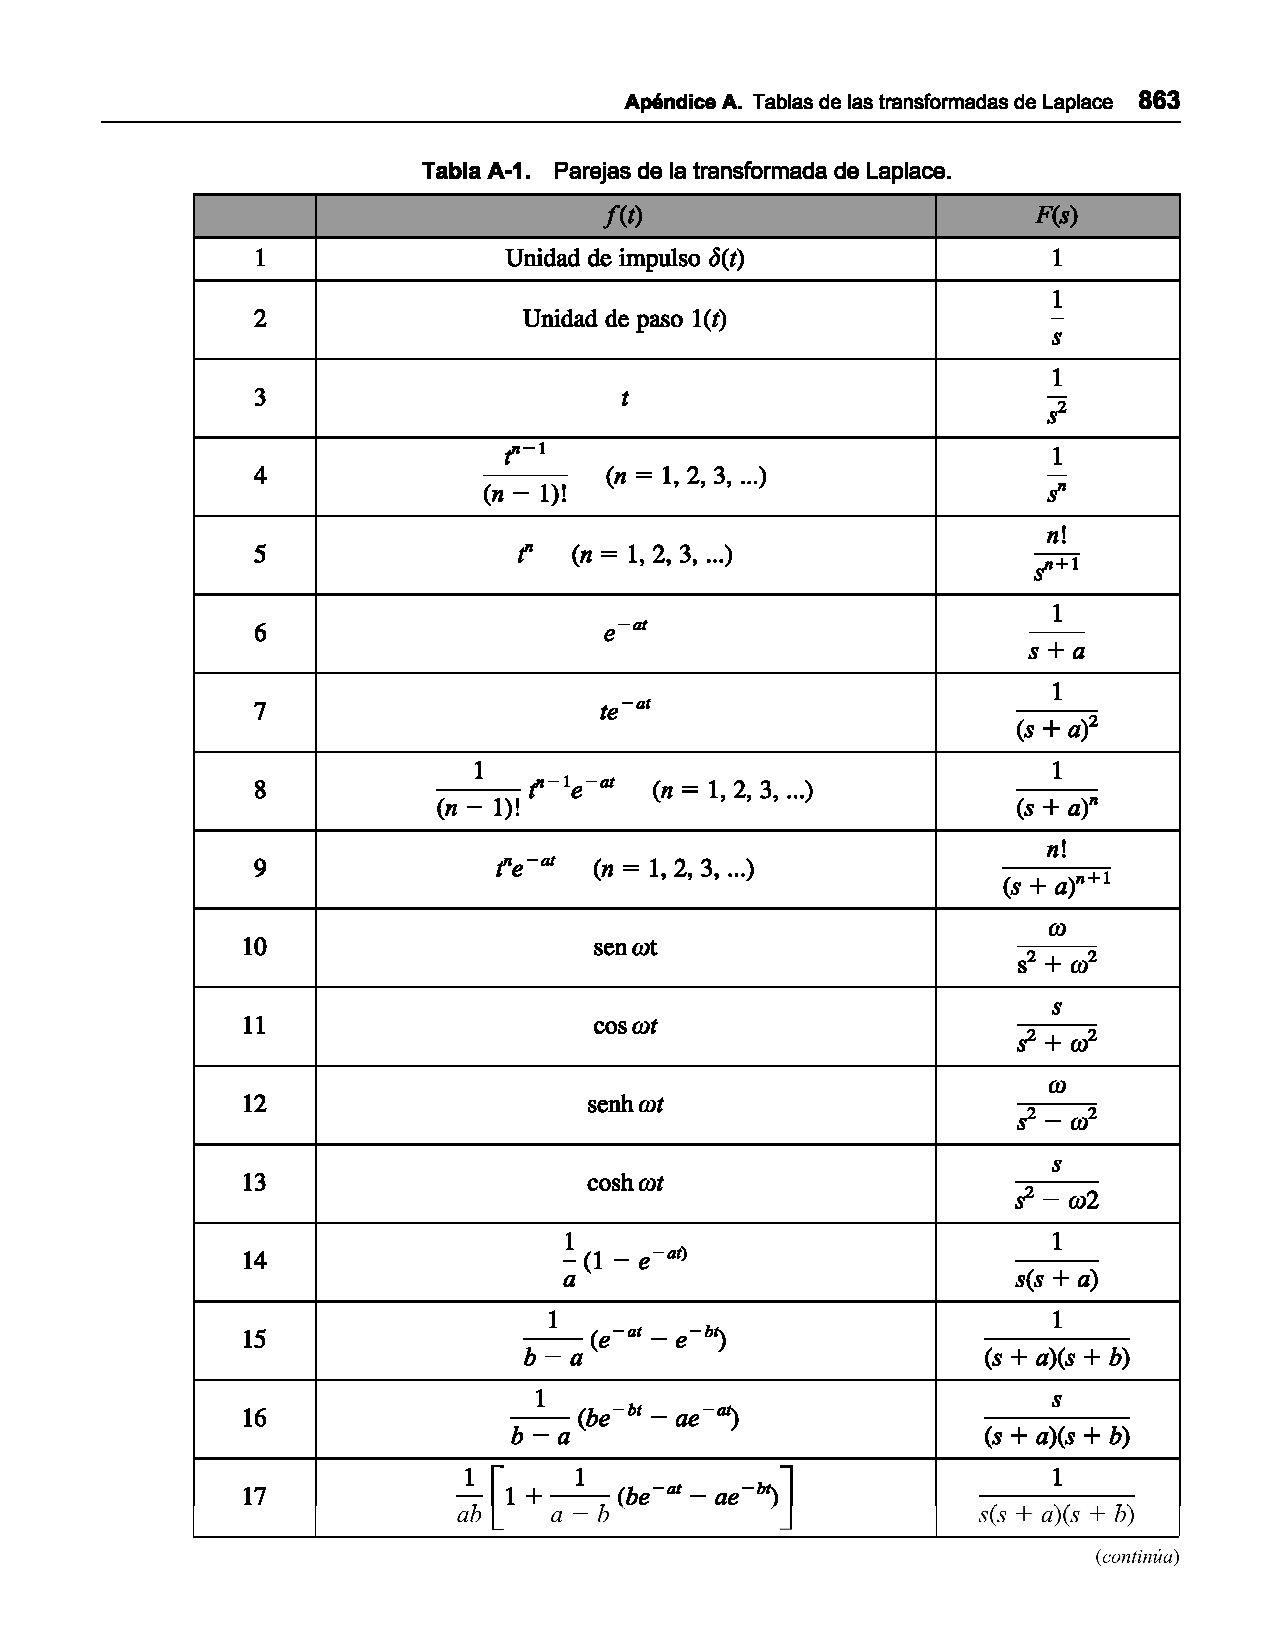
\includepdf[pages=-, pagecommand={}]{st/Laplace.pdf}
                    \newpage
                    \begin{multicols}{2}
                    \section{Señales y Sistemas}
                    
                    \subsection*{Funciones Básicas y Propiedades}
                    \begin{itemform}
                    \item \textbf{Par/Impar}:
                      $$x(-t)=x(t) \quad (\text{par}) \quad x(-t)=-x(t) \quad (\text{impar})$$
                    \item \textbf{Descomposición par/impar}:
                      $$x(t) = x_e(t) + x_o(t) $$
                      $$x_e(t)=0.5[x(t)+x(-t)] \quad (\text{par}) $$
                      $$x_o(t)=0.5[x(t)-x(-t)] \quad (\text{impar})$$
                    \item \textbf{Periodo fundamental}:
                      $$x(t)=x(t+T) \quad T=m\frac{2\pi}{\omega_0} $$
                    \end{itemform}
              
                    \fmSubSec{Transformaciones en el Tiempo}
                    \begin{itemform}
                    \begin{multicols}{2}
                    \item \textbf{Shift}:
                      $$y(t) = x(t - t_0) $$
                    
                    \columnbreak
                    \item \textbf{Mirror}:
                      $$y(t) = x(-t) $$
                    \end{multicols}
                    \item \textbf{Escalamiento}:
                      $$y(t) = x(at) \quad \text{Shrink if } |a| > 1, \text{ Xpand if } |a| < 1$$
                    \end{itemform}
                    
                    \fmSubSec{Señales Exponenciales y Sinusoidales}
                    \begin{multicols}{2}
                    \begin{itemform}
                    \item \textbf{Exponenciales}:
                      $$x(t) = e^{st}, s = \sigma + j\omega $$
                    
                    \columnbreak
                    \item \textbf{Sinusoidales}:
                      $$x(t) = A\cos(\omega t + \phi) $$
                    \end{itemform}
                        
                    \end{multicols}
                    
                    \fmSubSec{Impulso y Escalón Unitario}
                    \begin{itemform}
                    \item \textbf{Definiciones}:
                      $$\delta(t) = \frac{du(t)}{dt} \quad u(t) = \int_{-\infty}^t \delta(\tau)d\tau$$
                      $$\delta[n] = \begin{cases} 1 & n=0 \\ 0 & n\neq 0 \end{cases} \quad u[n] = \begin{cases} 1 & n\geq 0 \\ 0 & n<0 \end{cases}$$
                    \item \textbf{Propiedades de muestreo}:
                      $$x(t)\delta(t) = x(0)\delta(t) \quad x(t)\delta(t-t_0) = x(t_0)\delta(t-t_0)$$
                    \item \textbf{Representación de señales}:
                      $$x(t) = \int_{-\infty}^{\infty} x(\tau)\delta(t-\tau)d\tau $$
                    \end{itemform}
                    
                    
                    \fmSubSec{Sistemas LTI y Propiedades}
                    \begin{itemform}
                    \item \textbf{Linealidad}:
                      $$T\{a x_1(t) + b x_2(t)\} = a T\{x_1(t)\} + b T\{x_2(t)\}$$
                    \item \textbf{Invariancia temporal}:
                      $$\text{Si } T\{x(t)\} = y(t) \Rightarrow T\{x(t-t_0)\} = y(t-t_0)$$
                    \end{itemform}
                    \begin{multicols}{2}
                    \begin{itemform}
                        \item \textbf{Causalidad}:\\
                      Salida depende de entradas presentes
                      $$h(t) = 0 \ \forall t < 0 $$
                      
                    \columnbreak
                    \item \textbf{Estabilidad BIBO}:
                      $$\int_{-\infty}^{\infty} |h(t)|dt < \infty $$
                    \end{itemform}
                    \end{multicols}

                    \fmSubSec{Convolución}
                    \begin{itemform}
                    \item \textbf{Convolución continua y discreta}:
                      $$y(t) = x(t) * h(t) = \int_{-\infty}^{\infty} x(\tau)h(t-\tau)d\tau$$
                      
                    \item \textbf{Propiedades}:
                      \begin{itemize}[leftmargin=*,noitemsep,topsep=0pt]
                        \item Conmutativa: $x * h = h * x$
                        \item Asociativa: $x * (h_1 * h_2) = (x * h_1) * h_2$
                        \item Distributiva: $x * (h_1 + h_2) = x * h_1 + x * h_2$
                        \item Identidad: $x * \delta = x$
                      \end{itemize}
                    \end{itemform}
                    
                    \fmSubSec{Respuesta}
                    \begin{multicols}{2}
                        \begin{itemform}
                    \item \textbf{Al impulso}:
                      $$h(t) = T\{\delta(t)\} $$
                    
                    \columnbreak
                    \item \textbf{Sistema}:
                      $$y(t) = x(t) * h(t) $$
                    \end{itemform}
                    \end{multicols}
                    
                    \fmSubSec{Teorema de Muestreo}
                    \begin{itemform}
                    \item \textbf{Muestreo ideal}:
                      $$x_s(t) = \sum_{n=-\infty}^{\infty} x(nT)\delta(t-nT)$$
                    \item \textbf{Teorema de Nyquist}:
                      $$f_s > 2f_m \quad \omega_s > 2\omega_m \quad T < \frac{\pi}{\omega_m}$$
                    \end{itemform}
                    
                    \fmSubSec{Series de Fourier}
                    \begin{itemform}
                    \item Magnitud y Fase
                    $$|X(jw)|= \dfrac{1}{\sqrt{a^2+\omega^2}} \quad \angle X(jw)=-\arctan(\omega/a)$$
                    \item \textbf{Series exponencial compleja}:
                      $$x(t) = \sum_{k=-\infty}^{\infty} c_k e^{jk\omega_0 t} \quad c_k = \frac{1}{T} \int_T x(t)e^{-jk\omega_0 t}dt$$
                    \item \textbf{Forma trigonométrica}:
                      $$x(t) = a_0 + \sum_{k=1}^{\infty} [a_k\cos(k\omega_0 t) + b_k\sin(k\omega_0 t)]$$
                      $$a_0 = \frac{1}{T} \int_T x(t)dt, \quad a_k = \frac{2}{T} \int_T x(t)\cos(k\omega_0 t)dt$$
                      $$b_k = \frac{2}{T} \int_T x(t)\sin(k\omega_0 t)dt$$
                    \item \textbf{Coeficientes espectrales}:
                      $$|c_k|: \text{amplitud} \quad \angle c_k: \text{fase}$$
                    \end{itemform}
                    
                    \section{Transformada de Fourier}
                    \begin{itemform}
                    \item \textbf{Definición continua}:
                      $$X(\omega) = \int_{-\infty}^{\infty} x(t)e^{-j\omega t}dt$$
                      $$x(t) = \frac{1}{2\pi} \int_{-\infty}^{\infty} X(\omega)e^{j\omega t}d\omega$$
                    \item \textbf{Respuesta en frecuencia}:
                      $$H(\omega) = \int_{-\infty}^{\infty} h(t)e^{-j\omega t}dt \quad Y(\omega) = H(\omega)X(\omega)$$
                      
                    \end{itemform}
    \begin{itemform}
                        \item Linealidad: 
                        $$ax_1(t)+bx_2(t) \leftrightarrow aX_1(\omega)+bX_2(\omega)$$
                        \item Desplazamiento: 
                        $$x(t-t_0) \leftrightarrow X(\omega)e^{-j\omega t_0}$$
                        \item Convolución: 
                        $$x(t)*h(t) \leftrightarrow X(\omega)H(\omega)$$
                        \item Dualidad:
                        $$X(t) \leftrightarrow 2\pi x(-\omega)$$
                       \item 
    \end{itemform}


                    
                    \end{multicols}
                    
                    \begin{multicols}{2}

\subsection{Transformadas de Fourier}
$$
\begin{aligned}
  % Función constante (usando delta)
  \frt{1} &= 2\pi\delta(\omega)\\
  % Delta de Dirac
  \frt{\delta(t)} &= 1\\
  % Escalón unitario
  \frt{u(t)} &= \pi\delta(\omega) + \frac{1}{i\omega}\\
  % Exponencial causal
  \frt{e^{-at}u(t)} &= \frac{1}{a + i\omega}, \quad a > 0\\
  % Exponencial bilateral
  \frt{e^{-a|t|}} &= \frac{2a}{a^2 + \omega^2}, \quad a > 0\\
  % Pulso rectangular
  \frt{\text{rect}\left(\frac{t}{\tau}\right)} &= \tau\,\text{sinc}\left(\frac{\omega\tau}{2}\right)\\
  % Función sinc
  \frt{\text{sinc}(at)} &= \frac{\pi}{a}\text{rect}\left(\frac{\omega}{2a}\right)\\
  % Seno
  \frt{\sin(\omega_0 t)} &= \frac{\pi}{i}[\delta(\omega - \omega_0) - \delta(\omega + \omega_0)]\\
  % Coseno
  \frt{\cos(\omega_0 t)} &= \pi[\delta(\omega - \omega_0) + \delta(\omega + \omega_0)]\\
  % Gaussiana
  \frt{e^{-at^2}} &= \sqrt{\frac{\pi}{a}}e^{-\dfrac{\omega^2}{4a}}, \quad a > 0\\
  % Signo
  \frt{\text{sgn}(t)} &= \frac{2}{i\omega}\\
\end{aligned}
$$
\columnbreak

\subsection{Transformadas Inversas de Fourier}
$$
\begin{aligned}
  \frtn{\delta(\omega)} &= \frac{1}{2\pi}\\
  \frtn{1} &= \delta(t)\\
  \frtn{\pi\delta(\omega) + \frac{1}{i\omega}} &= u(t)\\
  \frtn{\frac{1}{a + i\omega}} &= e^{-at}u(t), \quad a > 0\\
  \frtn{\frac{2a}{a^2 + \omega^2}} &= e^{-a|t|}, \quad a > 0\\
  \frtn{\tau\,\text{sinc}\left(\frac{\omega\tau}{2}\right)} &= \text{rect}\left(\frac{t}{\tau}\right)\\
  \frtn{\frac{\pi}{a}\text{rect}\left(\frac{\omega}{2a}\right)} &= \text{sinc}(at)\\
  \frtn{\frac{\pi}{i}[\delta(\omega - \omega_0) - \delta(\omega + \omega_0)]} &= \sin(\omega_0 t)\\
  \frtn{\pi[\delta(\omega - \omega_0) + \delta(\omega + \omega_0)]} &= \cos(\omega_0 t)\\
  \frtn{\sqrt{\frac{\pi}{a}}e^{-\dfrac{\omega^2}{4a}}} &= e^{-at^2}, \quad a > 0\\
  \frtn{\frac{2}{i\omega}} &= \text{sgn}(t)\\
\end{aligned}
$$

\end{multicols}

\newpage
\begin{multicols}{2}
\textbf{Ziegler Nichols}

\begin{itemform}
  
  \item \textbf{Sigmoide}   
  
  (No aplica con integrador, ni polos $\mathbb{C}$ dominantes)
  $$G_c(s) = K_p\left(1 + \frac{1}{T_i s} + T_d s\right)$$
  $$K_P = 1.2 T/L \quad T_i = 2L \quad T_d = 0.5 L$$
  $$G_c(s)= 0.6 T \dfrac{(s+1/L)^2}{s}$$
  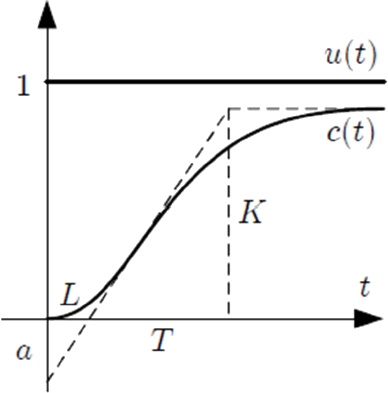
\includegraphics[width=0.5\linewidth]{src/Sigmoide.png}
  
  \item \textbf{Oscilación}
  $$G_C(s) = K_p$$
  $$K_P = 0.6 K_{CR} \quad T_i = P_{CR}/2 \quad T_d = P_{CR}/8$$
  $$P_{CR} = \frac{2\pi}{\omega_{CR}}$$
\end{itemform}


\textbf{Magnitud y Fase}
    $$
\left|H(j\omega)\right|=
\dfrac{\sqrt{ \text{Re} (N(j\omega))^2 + \text{Im} (N(j\omega))^2 }}
{\sqrt{\text{Re}(D(j\omega))^2+\text{Im}(D(j\omega))^2}} 
$$

$$
\angle N(j\omega)=
\tan^{-1}\left(
\frac{\text{Im}\{N(j\omega)\}}
{\text{Re}\{N(j\omega)\}}
\right)
$$

$$
\begin{aligned}
\angle \left(\dfrac{Num(j\omega)}{Den(j\omega)}\right)&=\tan^{-1}\left(
\frac{\text{Im}\{Num(j\omega)\}}
{\text{Re}\{Num(j\omega)\}}
\right)\\
&-\tan^{-1}\left(
\frac{\text{Im}\{Den(j\omega)\}}
{\text{Re}\{Den(j\omega)\}}
\right)
\end{aligned}
$$
\section{Diagramas de bode}
\begin{tabular}{|l|c|c|c|}
\hline
\textbf{Forma} & \textbf{dB/dec} & $w_{esq}$& \textbf{Extra} \\ \hline


$1/s$   & $20$  & N/A & $db |1/s| = 20$\\ 
        &       &     & $\angle (1/s)=-90$\\ \hline
$\dfrac{1}{\tau s+1}$ & $-20$ & $1/\tau$ & \\ \hline

$\dfrac{\omega_n}{(s^2+2 \zeta\omega_n s+\omega_n^2)}$
& $-40$
& $\omega_n$ &
\\ \hline

\end{tabular}
\subsection*{Lazo cerrado}

Con realimentación negativa unitaria:
\[
T(s)=\frac{G_c(s)G_p(s)}
{1+G_c(s)G_p(s)}.
\]


\section*{5. Márgenes de estabilidad}

Frecuencia de cruce de ganancia:
\[
|G(j\omega_{gc})|=1
\]
o equivalentemente
\[
M_{\mathrm{dB}}(\omega_{gc})=0\text{ dB}.
\]

Margen de fase:
\[
\boxed{
PM=180^\circ+\angle G(j\omega_{gc})
}
\]

Frecuencia de cruce de fase:
\[
\angle G(j\omega_{pc})=-180^\circ.
\]

Margen de ganancia:
\[
\boxed{
GM_{\mathrm{dB}}=-20\log_{10}|G(j\omega_{pc})|
}
\]

Si se usa la magnitud en dB directamente:
\[
GM_{\mathrm{dB}}=-M_{\mathrm{dB}}(\omega_{pc}).
\]


\end{multicols}
\newpage
% ============================================================
% SECCIÓN: Decibeles, Transductores, SPL y Señales
% ============================================================
\section{Decibeles, Transductores, SPL y Señales}
\begin{multicols}{2}

\textbf{Magnitud}
    $$
\left|H(j\omega)\right|=
\frac{\sqrt{\Re\{N(j\omega)\}^2+\Im\{N(j\omega)\}^2}}
{\sqrt{\Re\{D(j\omega)\}^2+\Im\{D(j\omega)\}^2}} 
$$
\fmSubSec{Decibeles y SPL}
\begin{itemform}
\item \textbf{Intensidad de sonido}
$$
I = \dfrac{P}{A} \quad  p = \text{ presión} 
$$
\item \textbf{Intensidad acustica}
$$
I = \dfrac{p^2}{2\rho c} \quad c = 344 \text{ m/s, }, \rho = \text{ densidad del medio} 
$$
  \item \textbf{dB}: 
$$A\log_{10}(P/P_0) \quad P_0 = 1\text{E-12}$$ 
$$A = 10 \text{ potencia, } 20 = \text{amplitud}$$

\item \textbf{SPL} 
$$SPL = 20\log_{10}(p_{rms}/p_0) \quad p_0 = 20\,\mu\text{Pa}$$

\item \textbf{Suma incoherente}: 

$$dB = 10\log_{10}\left(\sum 10^{dB/10}\right)$$



\end{itemform}


\fmSubSec{RLC: Función de Transferencia}
\begin{itemform}
\item Dominio $s$: 
$$R\rightarrow R \quad L\rightarrow sL \quad C\rightarrow 1/sC$$

\end{itemform}



\fmSubSec{Transformada de Laplace y DFT}
\begin{itemform}
  \item \textbf{Transformada de Laplace}:
  $$X(s) = \int_0^\infty x(t)e^{-st}dt \quad s = \sigma + j\omega$$
  \item \textbf{Transformada de Fourier}:
  $$X(j\omega) = \int_{-\infty}^{\infty} x(t)e^{-j\omega t}dt$$
  \item \textbf{Transformada de Fourier Discreta}:
  $$X[k] = \sum_{n=0}^{N-1} x[n]e^{-j2\pi kn/N}$$
\end{itemform}

\fmSubSec{Laplace, ROC y Estabilidad}
\begin{itemform}
\item $X(s)=\displaystyle\int_0^\infty x(t)e^{-st}dt$, \ $s=\sigma+j\omega$

\item \textbf{FT = Laplace en el eje $j\omega$}: $X(j\omega)=X(s)|_{s=j\omega}$ \textbf{solo si el eje $j\omega$ está en la ROC}

\item \textbf{Estabilidad BIBO} (causal): todos los polos con $\text{Re}(s)<0$ (semiplano izquierdo)

\item Polos de $s^2LC+sRC+1=0$: con $R,L,C>0$ siempre en semiplano izquierdo $\Rightarrow$ circuito RLC pasivo \textbf{siempre estable}

\item Regla: sustituir $s\rightarrow j\omega$ es válido \textbf{solo si el sistema es estable}
\end{itemform}


\columnbreak

% ============================================================
% COLUMNA 2
% ============================================================
\fmSubSec{Función Periódica y Envolvente}
\begin{itemform}
\item $x(t)=A\sin(\omega t+\phi)+DC$, \ $T=1/f$, \ $\omega=2\pi f$

\item \textbf{Partes}: amplitud $A$, fase $\phi$, offset DC, fundamental $f_0$ y armónicos $nf_0$

\item \textbf{Envolvente (ADSR)}: \textbf{Attack} (subida a pico) $\rightarrow$ \textbf{Decay} (baja a sostenimiento) $\rightarrow$ \textbf{Sustain} (nivel estable) $\rightarrow$ \textbf{Release} (caída a 0)

\item Obtención: rectificación + filtro pasa-bajas, o magnitud de la señal analítica (Hilbert)
\end{itemform}
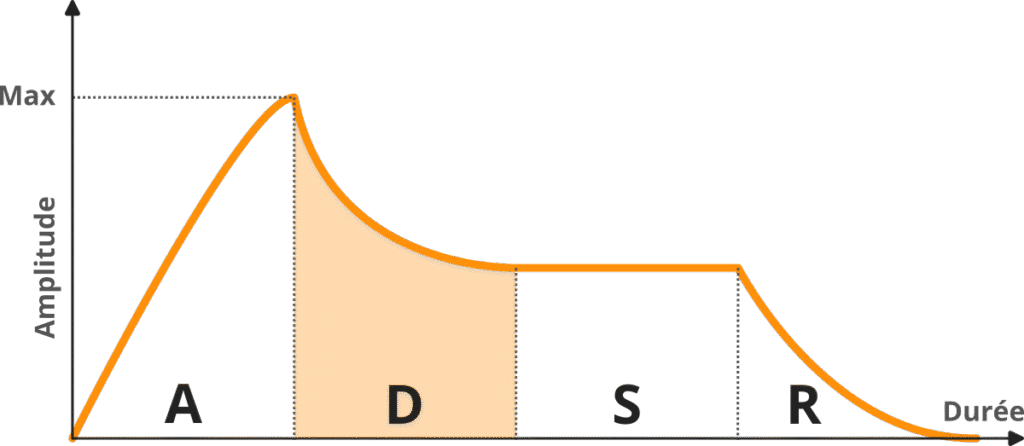
\includegraphics[width=0.6\linewidth]{src/Envolvente.png}

\fmSubSec{Microfonos}
\begin{itemform}
\item \textbf{Dinamico}
Consiste en una bobina móvil dentro de un campo magnético. 
No ocupa voltaje

\item \textbf{Condensador} 
Se utiliza un capacitor para captar la señal de entrada. Se ocupa
un voltaje para que jale

\end{itemform}
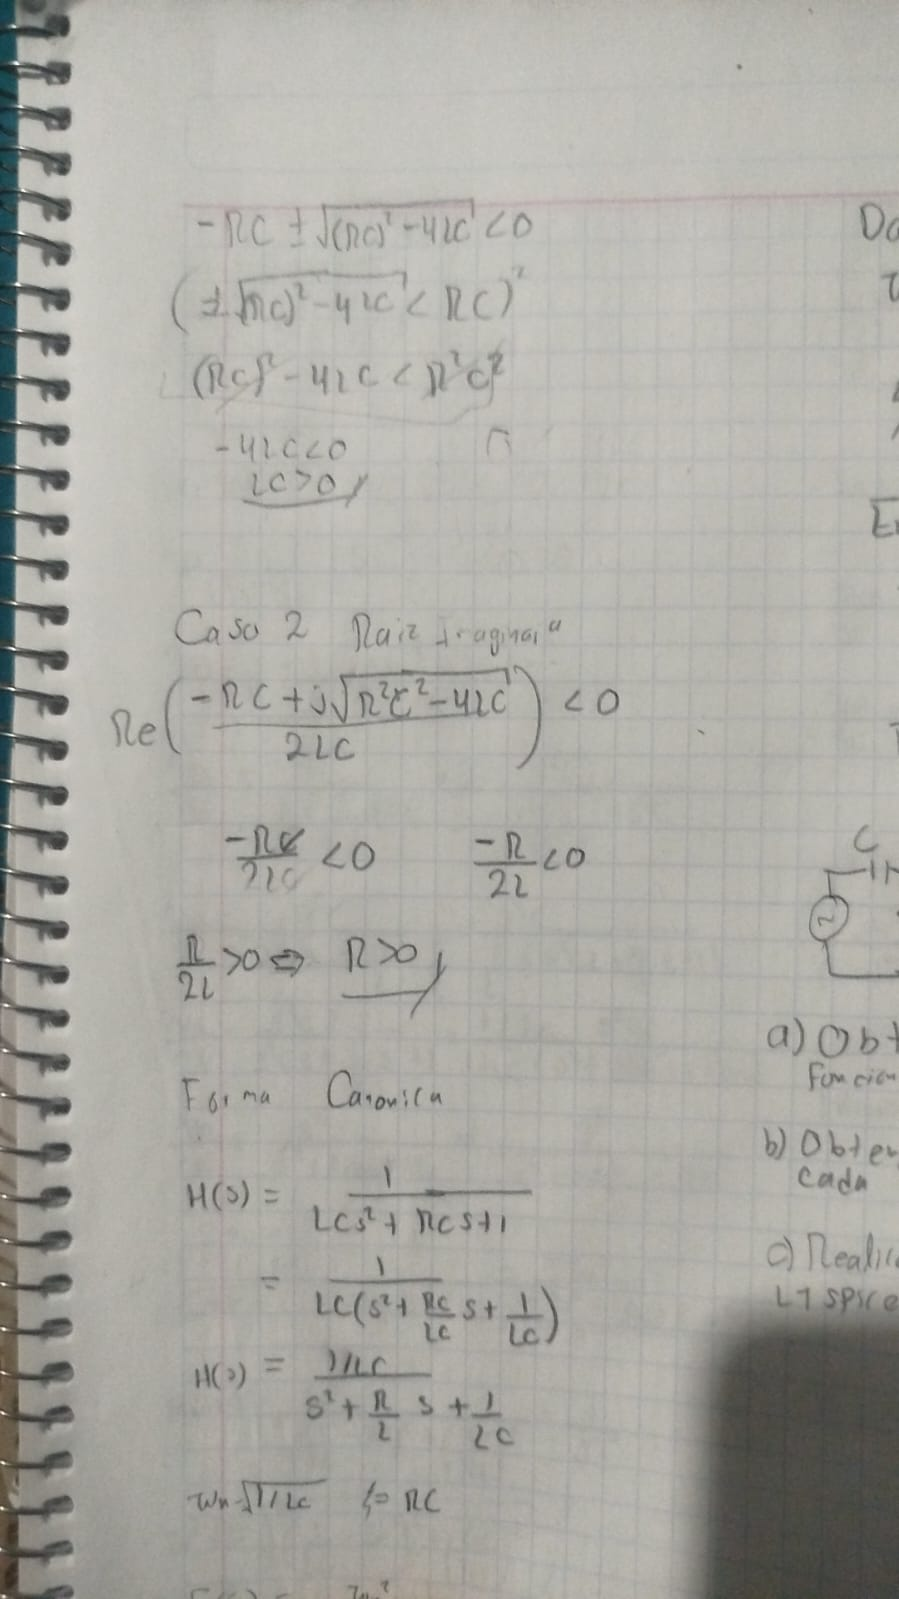
\includegraphics[width=0.7\linewidth]{src/Microfono.png}

\fmSubSec{CFT y DFT}
\begin{itemform}
\item \textbf{CFT}: 
Se aplica a señales continuas y de duración infinita. Se obtiene un espectro continuo.

\item \textbf{DFT}:
Se aplica a señales discretas y de duración finita. Se obtiene un espectro discreto y periódico. 

\item \textbf{CQT}:
Se aplica a señales discretas y de duración finita. Se obtiene un espectro discreto y no lineal (logarítmico).

\item \textbf{STFT}:
Cortar senales en segmentos

\end{itemform}





% ============================================================
% SECCIÓN: Crossover, EQ y RLC
% ============================================================

\fmSubSec{Crossover vs. Ecualizador}
\begin{itemform}
\item \textbf{Crossover}: filtros LP/HP/BP fijos que \textbf{enrutan} bandas a transductores distintos (woofer/tweeter); no cambia ganancia relativa, protege drivers

\item \textbf{Ecualizador}: ajusta \textbf{ganancia} (boost/cut) de bandas dentro del \textbf{mismo} camino de señal; da forma al tono. Sale una señal

\item \textbf{Clave}: crossover = enrutamiento espacial por banda $\quad$ EQ = conformado de ganancia
\end{itemform}

\begin{itemform}
  \item SubWoofer: 20-200 Hz (Muy Bajas Frecuencias)
  \item Woofer: 40-1000 Hz (Bajas Frecuencias)
  \item Midrange: 200-5000 Hz (Medias Frecuencias)
  \item Tweeter: 2000-20000 Hz (Altas Frecuencias)
\end{itemform}
\end{multicols}
\end{document}